\begin{figure}[htbp]
 \centering
 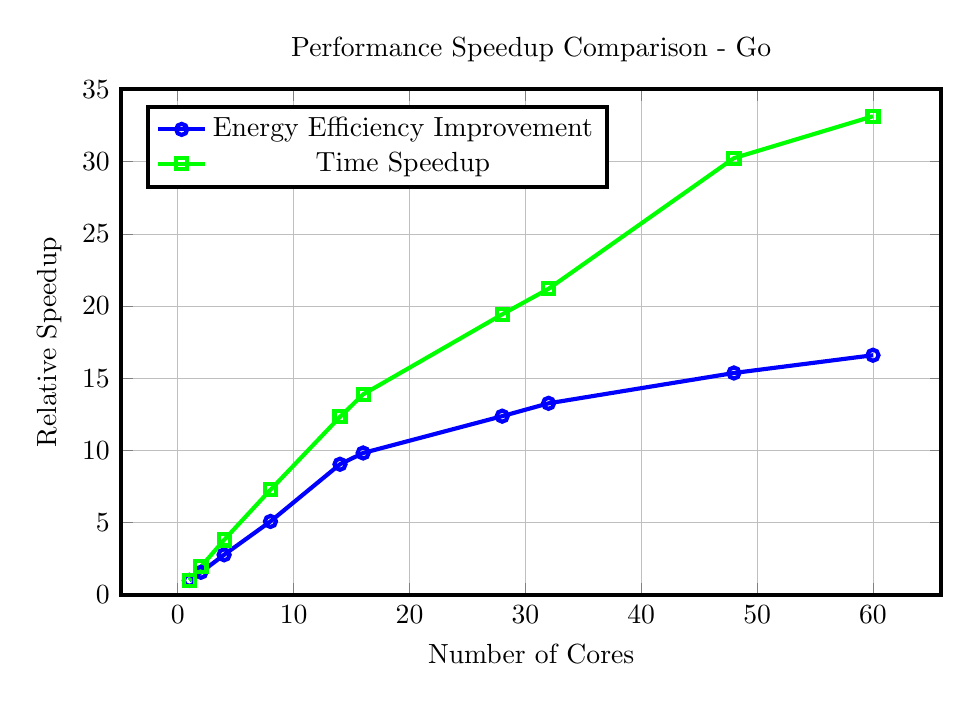
\begin{tikzpicture}
 \begin{axis}[
     xlabel={Number of Cores},
     ylabel={Relative Speedup},
     title={Performance Speedup Comparison - Go},
     grid=both,
     grid style={line width=.1pt, draw=gray!10},
     major grid style={line width=.2pt,draw=gray!50},
     width=12cm,
     height=8cm,
     legend pos=north west,
     mark size=2pt,
     line width=1.5pt,
     ymin=0,
     ymax=35
 ]
 
 % Energy speedup (selected points for clarity)
 \addplot[color=blue, mark=o] coordinates {
     (1, 1)
     (2, 1.56)
     (4, 2.77)
     (8, 5.08)
     (14, 9.04)
     (16, 9.82)
     (28, 12.37)
     (32, 13.26)
     (48, 15.36)
     (60, 16.59)
 };
 
 % Time speedup (selected points for clarity)
 \addplot[color=green, mark=square] coordinates {
     (1, 1)
     (2, 1.94)
     (4, 3.8)
     (8, 7.27)
     (14, 12.32)
     (16, 13.88)
     (28, 19.42)
     (32, 21.19)
     (48, 30.24)
     (60, 33.14)
 };
 
 \legend{Energy Efficiency Improvement, Time Speedup}
\end{axis}
\end{tikzpicture}
\caption[Go - Relative Performance Improvements]{Relative performance improvements showing time scales better than energy efficiency}\label{fig:go-routines-speedup}
\end{figure}

